\documentclass[12pt]{article}
\usepackage{fullpage}
\usepackage{graphicx}
\usepackage{subcaption}
\author{
Niraj Mahajan \\
\texttt{180050069} \and
Raaghav Raaj \\
\texttt{180050082}}
\title{CS 215 - Assignment 1}


\begin{document}
\maketitle
\section{Question 1}
\section{Question 2}
\section{Question 3}
\section{Question 4}



\newpage
\section{Question 5}
A sine wave of the form $y=5sin(2.2x + pi/3)$ is plotted, corrupted and filtered by three methods - moving median filtering, moving average filtering and moving quartile filtering and the \textbf{root mean squared errors} of the outputs of each method are : 
\begin{itemize}
\item 30 percent data corrupted
	\begin{enumerate}
	\item \textbf{Moving Median Filtering} = 28.121810
	\item \textbf{Moving Mean Filtering} = 99.607732
	\item \textbf{Moving Quartile Filtering} = 0.017173
	\end{enumerate}
\item 60 percent data corrupted
	\begin{enumerate}
	\item \textbf{Moving Median Filtering} = 692.400109
	\item \textbf{Moving Mean Filtering} = 351.490789
	\item \textbf{Moving Quartile Filtering} = 59.808615
	\end{enumerate}
\end{itemize}
The clean sine wave, corrupted wave, and the filtered waves using all three methods are plotted in Figure~\ref{fig:5.1} and Figure~\ref{fig:5.2}.

\begin{figure}[h!]
	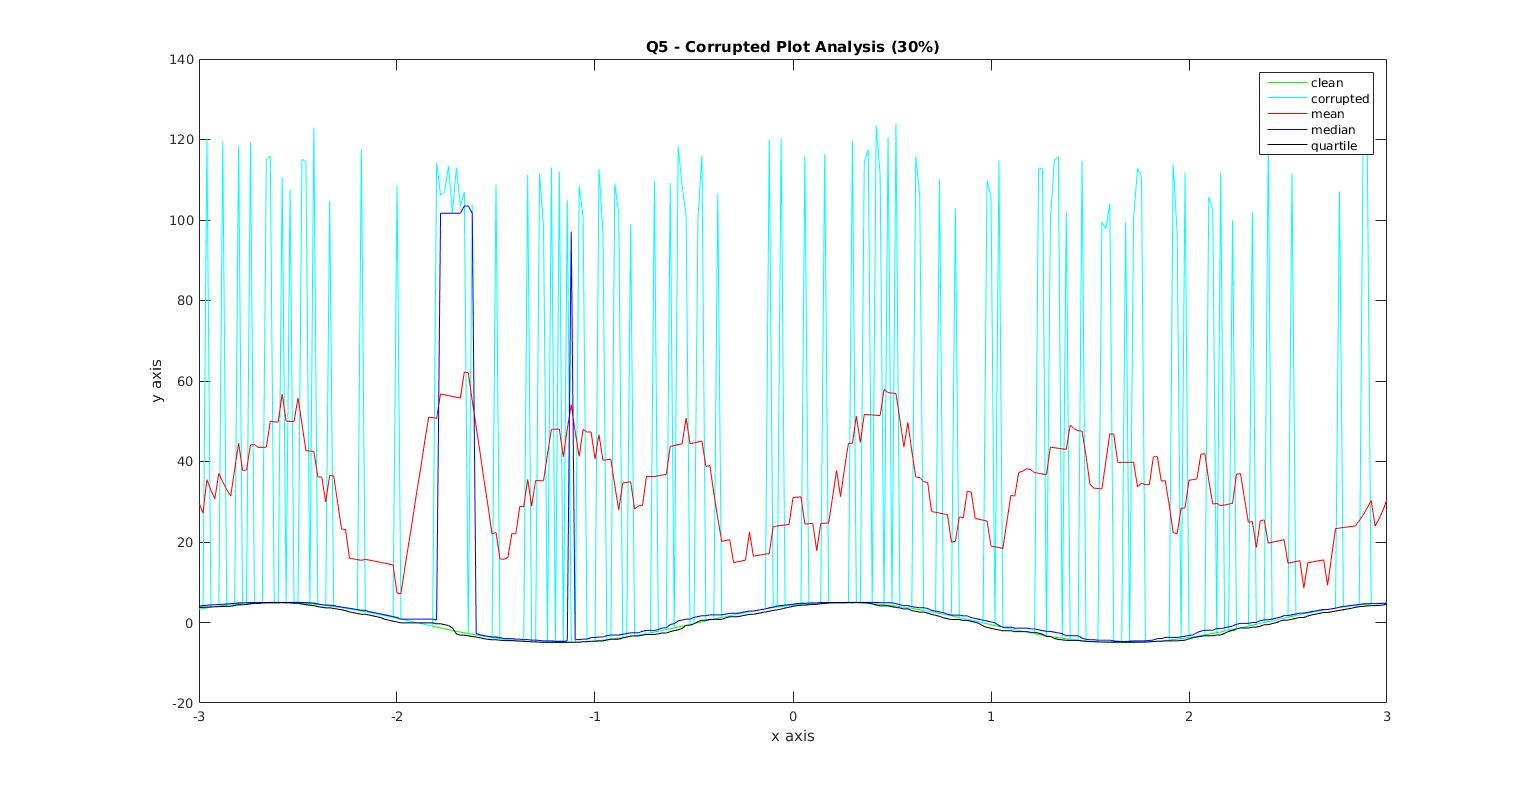
\includegraphics[width=\linewidth]{30.jpg}
	\caption{30\% data corrupted}
	\label{fig:5.1}
\end{figure}
\begin{figure}[h!]
	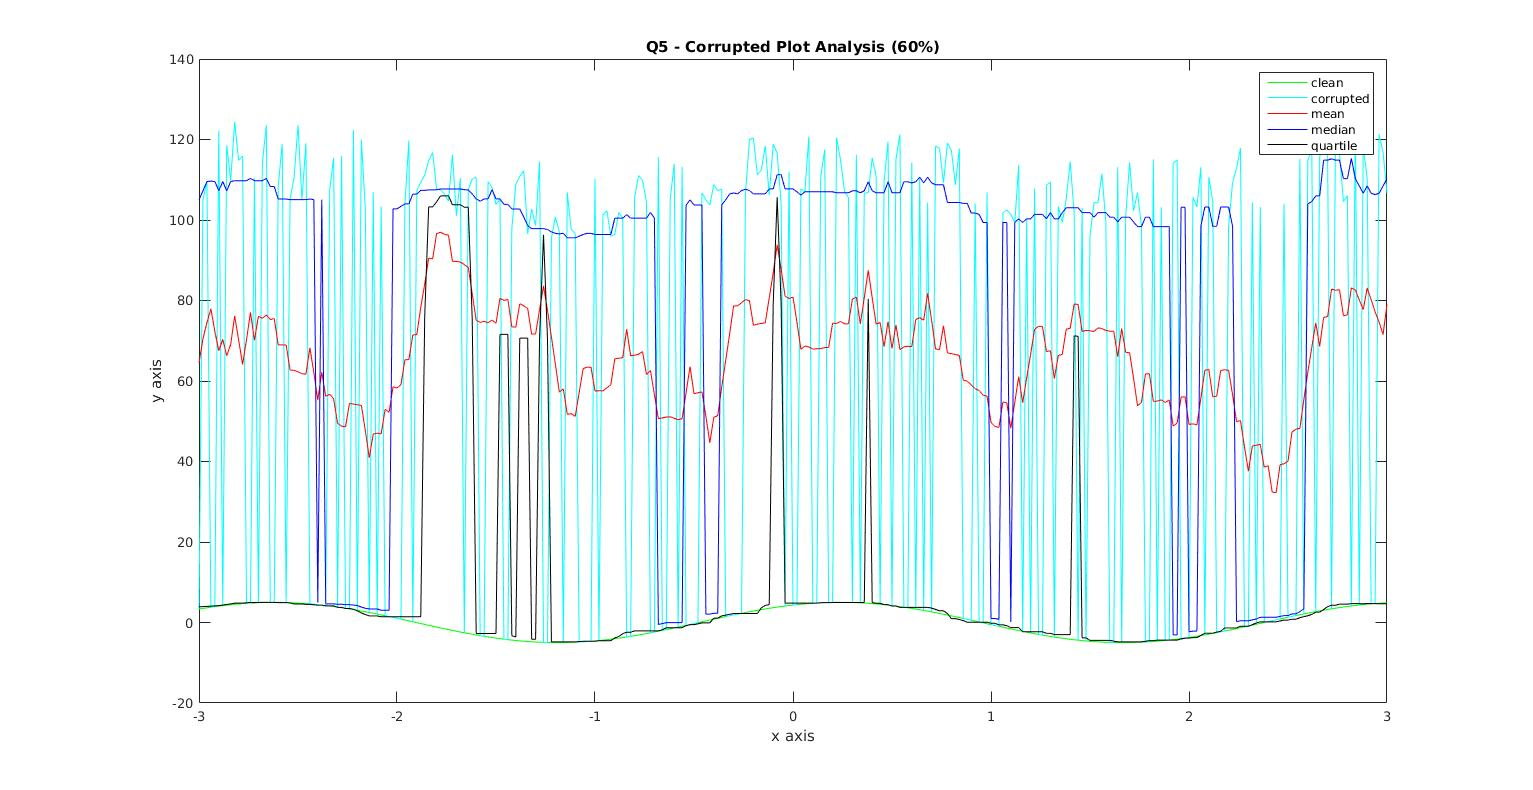
\includegraphics[width=\linewidth]{60.jpg}
	\caption{60\% data corrupted}
	\label{fig:5.2}
\end{figure}
\newpage
From the plots and the root mean square error data, it is clearly evident that the \textbf{moving quartile filtering} method has the \textbf{least root mean square error} and, hence, is the \textbf{best} method of filtering corrupted data.
\\ \\
This is because since the data is increased by around 100 when it is corrupted, we need to consider the smallest values in any interval while filtering. 


\textbf{Mean} of a data considers even the \textbf{corrupted values} and is heavily \textbf{influenced} by them. Hence we can safely rule out 'mean' as an optimum method for filtering.
 
 
\textbf{Median} of a data considers the middle term and is not influenced as heavily as mean by corruption but still, if \textbf{more than 50 \%} of the data is corrupted then the median will also be a \textbf{corrupted value}, and so we can rule out median as well.


\textbf{Quartile} of a dataset focusses on the lower 25\% data by value and we can say that it will \textbf{prioritize} \textbf{the clean (non corrupted) data} in any interval and hence will not get influenced by the corrupted data untill more than 75\% data in an interval has been corrupted.
\\ \\
\textbf{Hence moving quartile filtering is the best way to filter our data.}

\newpage
\section{Question 6}




\newpage
\section{Question 7}
\textbf{Formula}
\newline
The number of people 'n' such that any two of them have the same birthday with atleast 'p' probability is given by the inequality
$$\left(1-\frac{^{365}C_n}{365^n}\right) \leq p$$
The situation can be visualized as the negation of the event where all n people have unique birthdays.
\newline
The plot of values of n vs p is given in Figure~\ref{fig:7.1}
\begin{flushright}
$\forall$ p $\in \{5, 10, 15, 20, 30, 40, 50, 60, 70, 80, 90, 95, 99, 99.99, 99.9999, 100\}$
\end{flushright}
\begin{figure} [h!]
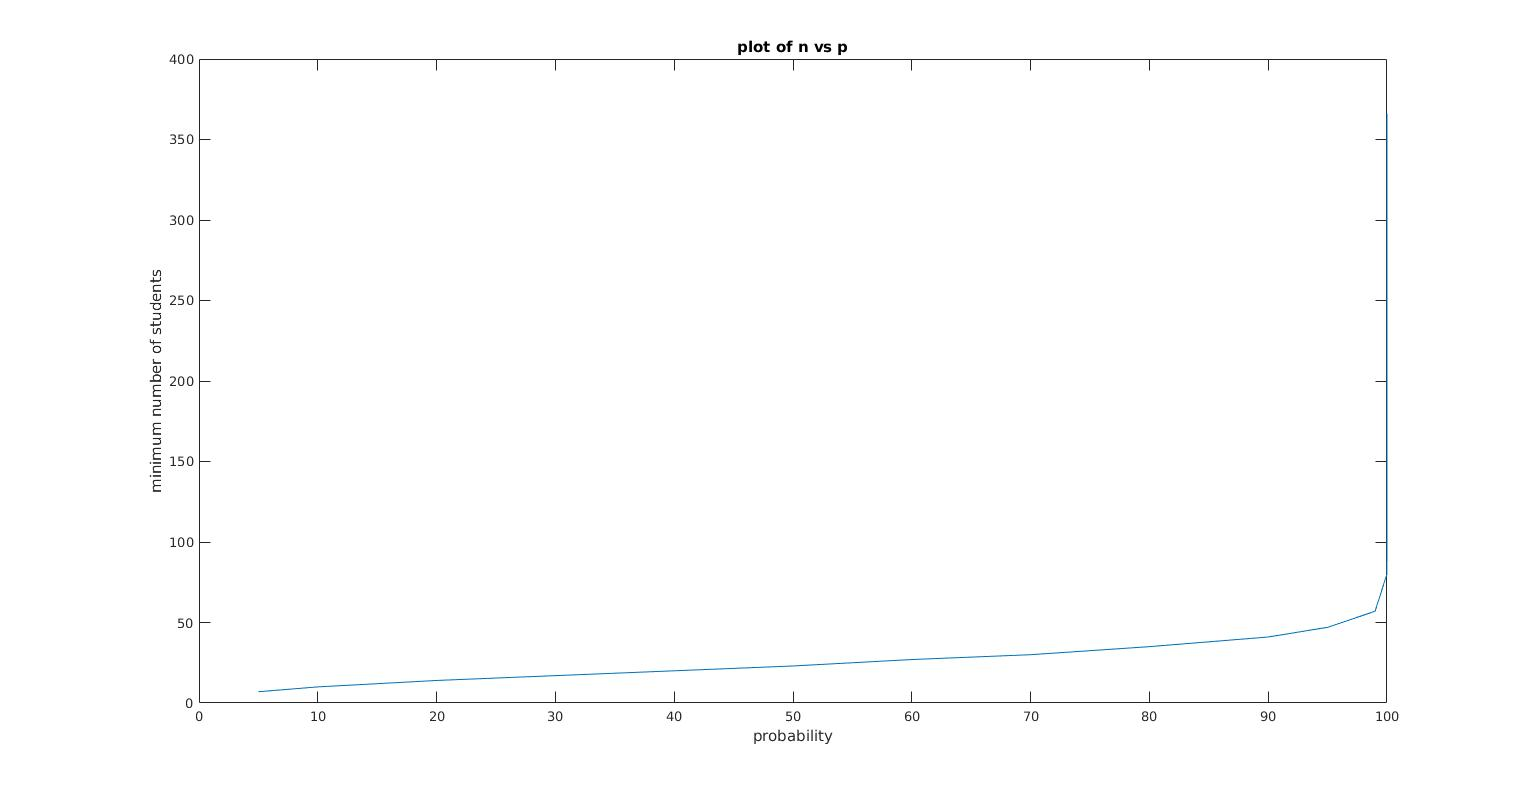
\includegraphics[width=\linewidth]{plot.jpg}
\caption{plot of n vs p}
\label{fig:7.1}
\end{figure}
\textbf{Usage of the MATLAB Code}
\begin{itemize}
\item Load code in the following path 'matlab\_code/q5/q5.m'
\item Run the code
\item This should output all values of n for corresponding values of p
\item This should also plot the required plot of n vs p
\end{itemize}

\end{document}